\chapter{Everyday life at university}

When you start your studies, you will be faced with new tasks and challenges that need to be mastered. The following pages will give you an impression of how your studies are structured and how learning at the university works.
But be sure to also read your Studienordnung~\link{https://www.verw.tu-dresden.de/AmtBek/PDF-Dateien/2016-06/11soBA24.04.2016.pdf}
and Prüfungsordnung~\link{https://www.verw.tu-dresden.de/AmtBek/PDF-Dateien/2016-06/11poBA24.04.2016.pdf}.

\minisec{Modules}
When you start your studies, you will be faced with new tasks and challenges that need to be mastered. The following pages will give you an impression of how your studies are structured and how learning at the university works. But be sure to also read your study regulations 58 and examination regulations 59.
Modules
In the course of your studies you have to successfully complete numerous so-called modules. A module can contain several courses. These can be lectures, tutorials, internships or seminars. Many modules consist of only one lecture and one tutorial. You complete a module by passing the module exam. A module examination can consist of one or more examinations (e.g. written examinations). Sometimes a preliminary examination must be passed before you are allowed to take part in the real exam. For the individual modules, Appendix 2 of the Studienordnung (Modulbeschreibung) specifies exactly which examinations must be taken.
Each module has a specified number of credit points (LP, often also called credits or ECTS points). One LP corresponds to a workload of 30 hours. If a module is worth 5 LP, this means that 150 hours of work are required over the course of the semester. This workload consists of attendance time (time you actually spend in lectures/tutorials at the university), time for preparation and follow-up of the courses (self-study), exam preparation and the exam itself. The LP for a module will be recognized after passing the module exam.

\minisec{Timetable}

At the university there is a so-called course schedule, which is published shortly before the beginning of each semester. You can find this list of courses, which is already sorted by semester, online on the Faculty's page~\link{https://www.inf.tu-dresden.de/}.
Your task is to create your own timetable from this list. For the beginning you will get ready-made timetables from us, from which you can then simply choose a timetable to enroll in jExam. Don't worry, we will do it together with you at ESE.

\pagebreak

While lectures generally have a fixed date, tutorials are flexible.
Simply register for the tutorials of your choice at jExam~\link{https://jexam.inf.tu-dresden.de/}.
However, if you find out later that your tutor has the qualities of a sleeping pill or that the tutorial is too full for you, do not hesitate to change it.

If you look at the available courses, you will come across the abbreviation SWS. SWS stands for Semesterwochenstunden and indicates the time required for a course. SWS is only a statement about the attendance time at the university. The time for preparation and wrap-up is not taken into account. 1 SWS means that the course is taught for an average of 45 minutes per week during the lecture period. A course with 4 SWS is taught for 3 hours per week. A teaching unit at the university lasts 90 minutes and is called a Doppelstunden (DS). A course with 4 SWS is therefore taught 2 times a week. It is a bit more complicated if a course is actually only 1 SWS. In this case, the course only takes place every 14 days and you have to check exactly whether the course takes place in even or odd calendar weeks. In the timetable you will then find the designations \enquote{1st\ week} or \enquote{2nd\ week}. These have nothing to do with the weeks relative to the beginning of the semester! \enquote{1st\ week} means that the course takes place in every odd calendar week and \enquote{2nd\ week} stands for even calendar weeks.
\begin{figure}
	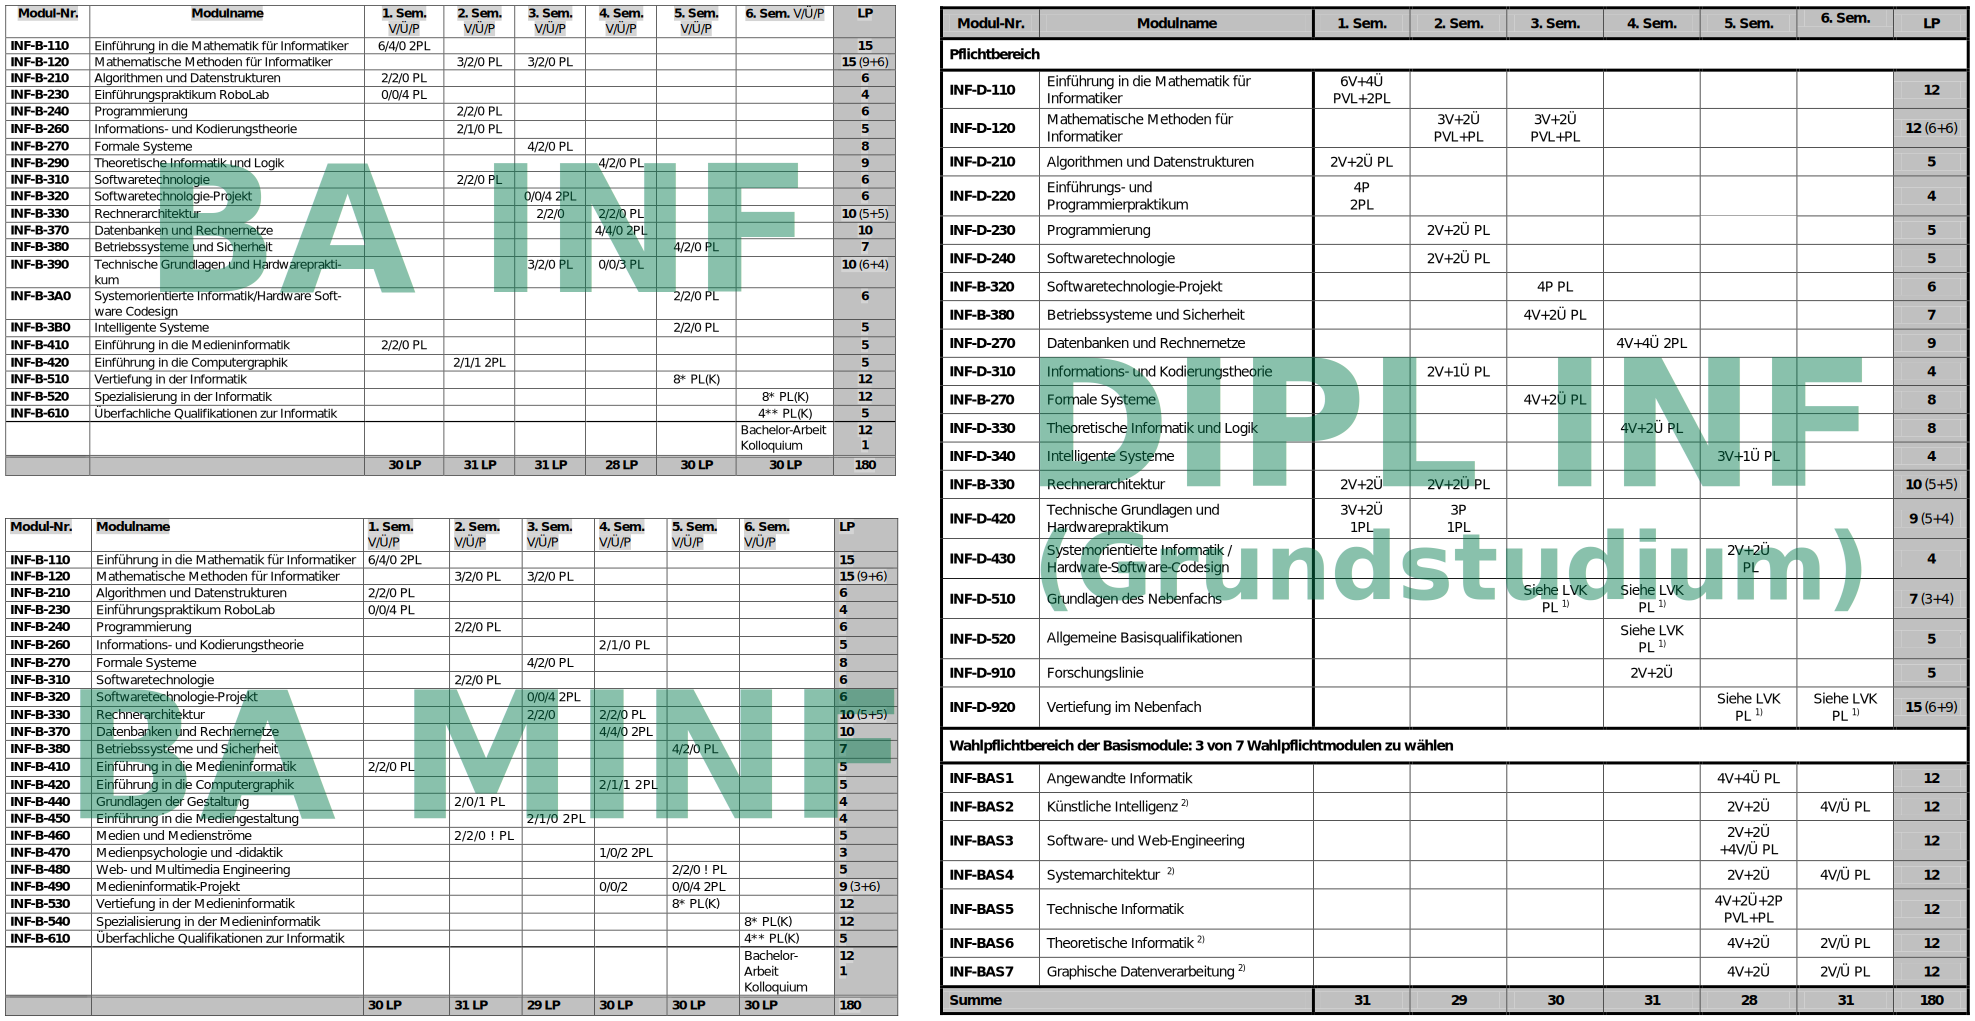
\includegraphics[width=\textwidth]{img/alle_studienablaufplaene.png}
	\caption*{\small \textit{Die Studienablaufpläne aller Studiengänge findest du in groß unter}~\link{https://tu-dresden.de/ing/informatik/studium/studienangebot}.}
\end{figure}

\minisec{Lecture}

In the lecture, the material is taught that will ultimately be asked in the exam. It is therefore advisable to actively follow the lecture and, if necessary, to prepare and follow up on it. It is not advisable to catch up on all the material before the exam, as the amount of material is usually very large and it would mean unnecessarily more stress during the exam phase.
\\
Especially at the beginning of your studies, the number of people attending a lecture is in the triple digits. Usually you will get used to this quickly. However, the more people there are in a lecture, the more likely it is that someone will not be able to keep up at some point in the lecture. This can happen to anyone. So if you are that someone, don't be shy about asking the lecturer a question. Active participation in the lecture is always appreciated by the lecturers. And yes, even if it is a question of understanding. Your fellow students who had the same question but didn't have the courage to ask will be happy. \\
Which lecture you should attend in which semester can be found in the respective study plan of your study program
(Bachelor Informatik~\link{https://www.verw.tu-dresden.de/AmtBek/PDF-Dateien/2016-06/11soBA24.04.2016.pdf}, Bachelor Medieninformatik~\link{https://www.verw.tu-dresden.de/AmtBek/PDF-Dateien/2016-06/11soBAMI24.04.2016.pdf}, Diplom Informatik~\link{https://tu-dresden.de/die_tu_dresden/fakultaeten/fakultaet_informatik/studium/dateien/studien_und_pruefungsordnungen/dipl_inf_so_app1_de.pdf}) or in the course catalog on the page of the faculty~\link{https://tu-dresden.de/ing/informatik/studium/lehre}. 


\minisec{Tutorial}

Tutorials are offered for almost all lectures and serve to work on tasks related to the current lecture material. Exams are often based on the tutorials, so you should visit the tutorials regularly. The tutorials are usually held by students from higher semesters or by faculty members, not by the professor. This also has the advantage that you understand many things better when they are explained to you by someone else. You can find the current tutorials on the page of the respective lecturer, often under the headings Teaching or Lehre. It is expected that you look at the exercise sheets before the tutorial in order to discuss solutions or questions.


\minisec{Internship}

The first internship awaits you during the lecture-free period of the first semester -- so don't plan your vacation too quickly! There you will prove your skills in the introductory internship \textit{Robolab}. Diploma students must also complete the Strategiespiel internship. A full internship semester is only mandatory for diploma students in the 7th semester. Of course, it is still advisable to do internships at real companies outside the faculty during the semester break. This not only increases your job chances, but also shows you whether your choice of study was really the right one.

\refstepcounter{dummy}\label{sec:pruefungen}
\minisec{Exams}
The exam period follows directly after the lecture period - probably the most stressful time in a student's life. You can find the exact exam dates for the winter semester usually around the beginning of January on the homepage of the faculty~\link{https://tu-dresden.de/ing/informatik/studium/news} or directly at the Prüfungsamt~\link{https://tu-dresden.de/ing/informatik/studium/pruefungsorganisation}.
During the semester you have the opportunity to register for the exam (within the registration period) via jExam.
here you also have the possibility to deregister up to three \emph{working} days before the exam. You can also take the exam in a later semester. Of course, this should not become the rule. For oral and other exams there is a withdrawal period of 14 days.
If you have to withdraw from the exam due to a sudden illness, you can find out on the website of the examination office which certificates you have to submit to the Prüfungsamt within which time limit ~\link{https://tu-dresden.de/ing/informatik/studium/pruefungsorganisation/pruefungen/abmelden-ruecktritt-krankheit}.
Exams are graded with grades, and all exams graded better than 5.0 are considered passed and cannot be repeated. Grades worse than 5.0 do not exist. Thus, a 5.0 is the only chance you have to fail an exam. Once you have done that, there is the possibility to repeat the exam within two semesters. After the second failed exam attempt, you only have one semester until the third one has to be taken. Only when you have failed the exam for the third time (i.e. the second retake), you will be exmatriculated. More detailed information on this topic can always be found in the Prüfungs- bzw.\ der Studienordnung, which you should definitely have a look at.
By the way, your first math exam is already waiting for you in December: the so-called Santa Claus exam.

\includegraphics{img/nikolauspruefung.png}

\minisec{certificate of achievement}

For some exams, you will receive a certificate of achievement (or Schein in short) in addition to your grade. These include language courses, the research line, and in some cases minor subject examinations. You need these certificates in order to be able to have these achievements credited to you in the Prüfungsamt.

\refstepcounter{dummy}\label{sec:sprachausbildung}
\minisec{Language courses}

Courses for almost all possible (and impossible) languages are offered at the TU Dresden. For this purpose there are two centers for language education: The \enquote{Lehrzentrum Sprachen und Kulturen} (LSK) and \enquote{TUD Institute of Advanced Studies} (TUDIAS).
DThe language courses offered by the two institutions are very similar. You have a budget of Semesterwochenstunden (10 SWS in total) for various language courses, which you can spend as you wish. For your bachelor studies in (Medien-)Informatik, language courses are generally optional, but definitely recommended. For diploma students, 2 semesters of English are mandatory during the course of studies. However, if you study Bachelor Informatik and want to continue with the Master Informatik at the TU Dresden afterwards, you will have have a proof of a B2 level in English, so it might be a good idea for you to attend the corresponding language courses. The enrollment for a language course is done online~\link{https://sprachausbildung.tu-dresden.de} with your ZIH login.
As soon as the courses are activated, you should hurry, because the popular courses are usually full within a few minutes. You can find more information on~\link{https://tu-dresden.de/lsk}~and~\link{https://www.tudias.de/}.


\minisec{Writing Consultation}
The Schreibzentrum of the TU Dresden~\link{https://www.facebook.com/SchreibzentrumTUD} is a cooperative project for students and teachers of the Center for Continuing Education and the Career Service. It offers support, methods and ideas on the topic of \enquote{scientific writing}.
You can either come to the open writing consultation hour at the SCS ServicePoint of the SLUB with your writing projects of all kinds (voucher, seminar paper, thesis, etc.) or make an individual appointment by e-mail~\link{mailto:Schreibzentrum@mailbox.tu-dresden.de}.
It does not matter how far along the work is, i.e. whether you are still at the very beginning or shortly before submission. It is also not necessary to have a concrete problem, but intuitive concerns about the work can also be provided.

The writing consultation supports you in questions about the writing process -- from finding a topic, to the outline, to the submission of the finished work. Trained student writing tutors support you with a variety of writing methods and techniques. They cannot give you tips on the content of your paper or help you with it. The writing tutor will also not proofread any texts; however, you can receive exemplary text feedback on text excerpts. The offer is of course free of charge.

\minisec{Scholarships}

In addition to BAföG, scholarships are also a popular way of financing your studies.

Many scholarships are awarded by the 13 mainly state-funded scholarship organizations, which differ in terms of their ideological, religious or political profile. Students are often recommended directly by schools, examination offices or university teachers on the basis of good performance. However, self-applications are also possible for many works. You by no means have to be an overachiever for admission.

Social commitment can play an equally important role in the selection process. The scholarships are calculated in accordance with BAföG, depending on the student's own income and assets as well as the income of his or her parents. In addition, scholarship holders receive a monthly flat-rate tuition fee of 300 euros. In contrast to BAföG, however, the scholarships do not have to be repaid. In addition to financial support, all works offer extensive non-material support in the form of language courses, excursions and academies.

Equally well-known is the Deutschlandstipendium, which is half financed by private donors. The financial support is independent of the student's income or that of his or her parents and amounts to 300 euros per month. The Deutschlandstipendium does not count towards BAföG and does not have to be repaid. Applications are accepted directly by the Zentrum für Weiterbildung der TU Dresden~\link{https://tu-dresden.de/deutschlandstipendium} in July.

There are many other organizations whose support is mainly privately financed. However, these often award only a few full scholarships or limit the funding to smaller contributions in kind or money. An overview of the multitude of funding possibilities can be obtained with the help of the scholarship database of the BMBF~\link{https://www.stipendienlotse.de}.

\begin{figure}[b]
	\centering
	\includegraphics[width=\textwidth, keepaspectratio]{img/xkcd/zealous_autoconfig.png}
	\caption*{{\small \textit{I hear this is an option in the latest Ubuntu release. (https://xkcd.com/416)}}}
\end{figure}

\minisec{University groups}
\label{sec:hsg}

Learning and partying are not enough for you? Find a university group! There you will find volunteer students who want to actively shape life on campus. And depending on what you are looking for, you will also be able to find discussions, the opportunity to help others, new experiences, interesting people and much more.

Thematically, there is something for everyone. There are university groups with political and social commitment. Others are interested in shaping cultural diversity in Dresden. Of course, there are also technically oriented university groups. Just have a look around here~\link{https://www.stura.tu-dresden.de/hochschulgruppen} and contact the university group of your choice directly. Maybe there is something for you.
Vielleicht ist ja was für dich dabei.

\minisec{Study abroad}

If you have an acute desire to go abroad or an urge to internationalize during your studies, please ask the university's international office or your professor of confidence. Stays abroad can cause side effects. You can ask fellow students about theirs.

In the course of your studies, people will ask you again and again whether you would like to spend one or two semesters abroad.
Now you may ask yourself as an innocent freshman, why do that and why are you coming up with it now?
Die Antwort ist einfach:
The answer is simple:
For one, you can directly improve your language skills, socialize and experience new cultures -- A welcome change to clear your head after the exhausting semesters. It gives you new perspectives, both academic and professional. It also helps you develop your soft skills such as independence, tolerance, and adaptability (to name a few). All things that will help you and you will be grateful for later on.
In short, a stay abroad is useful, but requires some planning.
Therefore it is advantageous to inform yourself as early as possible.
For information and if you have any questions, you can contact the International Office (AAA) of the TU~\link{https://tu-dresden.de/studium/im-studium/beratung-und-service/akademisches-auslandsamt} and visit the pages of the faculty~\link{https://tu-dresden.de/ing/informatik/studium/internationales/outgoing}.
If you are brave, you can even ask professors directly if they have contacts to other universities or companies.
It's up to you how successful your stay abroad will be.
Whether it's petting seals off Newfoundland or attending a scrum meeting in Silicon Valley, there are plenty of offers waiting for you!

% \begin{figure}[b!]
% 	\centering
% 	\includegraphics[width=0.9\linewidth]{img/ese2014/einschreibung.jpg}
% \end{figure}%

\minisec{Leave of Absence}
There are a number of reasons that can prevent you from properly continuing your studies at the TU. Classic reasons are serious illnesses, longer internships, stays abroad or (unexpected) offspring that you have to take care of. In such cases, you can take a leave of absence from your studies in order to fully concentrate on the reason for your leave. During a semester of leave, you are exempt from having to take exams, but you continue to enjoy all the benefits of being a student. On the other hand, you are usually not entitled to BAföG or child benefit payments during this time, so don't necessarily plan for this in your income.

If you study abroad and spend a few semesters in far-away countries, you can have your achievements and exams credited here. The only pitfall is that if you earn enough credits, you will still be advanced by one semester, but the student advisor can help you with that.

You can apply for a leave of absence at the Immatrikulationsamt~\link{https://tu-dresden.de/imma/} during the re-registration period for the next semester. You can find out exactly how to do this and further information under~\link{https://tu-dresden.de/studium/im-studium/studienorganisation/beurlaubung}.
